
\documentclass[man]{apa6}


\usepackage[american]{babel}

\usepackage{csquotes}

\usepackage{enumerate}
\usepackage{graphicx}
\usepackage{subfigure}

\usepackage{amsmath}

\usepackage[style=authoryear,sortcites=true, sorting=nyt, backend=biber, uniquename=false, uniquelist=false]{biblatex}
\DeclareLanguageMapping{american}{american-apa}

\addbibresource{literature.bib}


\DeclareMathOperator*{\argmin}{arg\,min}

\title{Human Search for a Target on a Textured Background is Consistent with a Stochastic Model}

%\textsuperscript{*}
\fourauthors{Alasdair D. F. Clarke}{Patrick Green}{Mike J. Chantler}{Amelia R. Hunt}
\fouraffiliations{School of Psychology, University of Aberdeen, Aberdeen, UK}{School of Mathematical and Computer Sciences, Heriot-Watt University, Edinburgh, UK}{School of Life Sciences, Heriot-Watt University, Edinburgh, UK}{School of Psychology, University of Aberdeen, Aberdeen, UK}


\shorttitle{Stochastic Search}

\begin{document}

\abstract{
Previous work has demonstrated that search for a target in noise is consistent with the predictions of the optimal search strategy, both in the spatial distribution of fixation locations and in the number of fixations observers require to find the target. In this manuscript we describe a challenging visual search task and compare the number of fixations required by human observers to find the target to predictions made by a stochastic search model. This model relies on a target visibility map based on human performance in a separate detection task. If the model does not detect the target, then it selects the next saccade by randomly sampling from the distribution of saccades that human observers made. We find that a memoryless stochastic model matches human performance in this task. Furthermore, we find that the similarity in the distribution of fixation locations between human observers and the ideal observer does not replicate: we find that rather than making the signature doughnut-shaped distribution predicted by the ideal search strategy, the fixations made by observers is best described by a central bias. We conclude that, when searching for a target in noise, humans use an essentially random strategy, which achieves near optimal behaviour due to biases in the distributions of saccades we have a tendency to make. The findings reconcile the existence of highly efficient search human performance with recent studies demonstrating clear failures of optimality in single and multiple saccade tasks.}
%246

\maketitle

% \linenumbers

%%%%%%%%%%%%%%%%%%%%%%%%%%%%%%%%%%%%%%%%%%%%%%%%%%%%%%%%%%%%%
% \section{Introduction}
%%%%%%%%%%%%%%%%%%%%%%%%%%%%%%%%%%%%%%%%%%%%%%%%%%%%%%%%%%%%%
The human retina provides highly accurate and detailed central vision, but acuity diminishes rapidly with eccentricity. Eye movements shift new locations to central vision, and in doing so sequentially sample finer-grained details from locations that are likely to yield important information, presumably using some combination of peripheral visual signals, inferences based on context, and top-down strategies. Each eye movement during extended search can therefore be useful for understanding how the visual system combines and prioritises information both within each fixation and across a sequence of fixations.

Much of the research on visual search to date has formalised this general issue by focusing on questions of  \itshape feature extraction \normalfont  and of \itshape strategy\normalfont. Feature extraction includes both top-down guided search \parencite{wolfe2007, zelinsky2008} and stimulus-driven (saliency) effects \parencite{itti-koch2000, gao2008, itti-baldi2009}.  For the abstract and discrete search items commonly used as visual search stimuli, categorical features such as colour, orientation, shape and size are often used. Simple qualitative comparisons between the search items and the target can be used to model top-down guidance \parencite{pomplun2003, rutishauser-koch2007}. For more complex stimuli, such as a target hidden in image noise or in a photograph of a natural scene, there is no discrete set of items to consider and more sophisticated image processing techniques are required \parencite{rao2002, zelinsky2008, pomplun2007,  hwang2009, tavassoli2009}. In either case, the output of a feature extraction mechanism is an activation map; that is, a representation of the visual array in which peaks of activity represent the priority of locations for eye movements.

Strategy refers to the mechanism for selecting which location to inspect next. While a number of different mechanisms have been put forward, the most commonly implemented has been the Maximum A Posteriori (MAP) observer. The MAP observer directs saccades to the current maximum of the activation map and a simple inhibition of return (IOR) mechanism is used to stop the model returning to previously fixated maxima. Depending on the model, a maximum will either represent a search item, or the centre of gravity of a number of search items. As most previous computational models have primarily been interested in the feature extraction stage of search, the MAP observer has often been used for simplicity \parencite{itti-koch2000, rao2002, pomplun2003, rutishauser-koch2007, clarke2009, zelinsky2008}.

An alternative to the MAP Observer is the Ideal Observer. Here, eye movements are directed to locations that are likely to yield the most information. An example of an Ideal Observer model comes from \textcite{najemnik-geisler2005}, who measured visual sensitivity to a Gabor patch in varying amounts of noise across a range of eccentricities and angles from fixation. From the visual sensitivity data they could generate a model of optimal eye movement behaviour that selected as the next fixation the location that would maximize the probability of detecting the target, given the amount of background noise and the known visibility of the target at various eccentricities. The number of fixations made during search for the target by the human observers (the two authors) closely matched the optimal model. In a second study \parencite{najemnik-geisler2008} they also measured the fixations generated by an optimal model and found that, when averaged over all trials, the Ideal Observer matched the human spatial distribution of fixations: both the model and human observers exhibited a preference for fixating above and below the centre of the image. The idea that eye movements during search are near-optimal is broadly consistent with studies demonstrating the speed and efficiency with which eye movements can be directed to locations in a naturalistic setting that provide the most task-relevant information. A now-classic example is the demonstration of expert cricket batsmen's ability to shift their eyes rapidly to the anticipated bounce point of the ball based on its trajectory as it leaves the bowler's hand \parencite{land2000}. This is a specific example of a number of studies demonstrating that eye movements are tightly constrained by task goals, and driven to maximise task-relevant information gain (for a recent review, see \textcite{hayhoe2014}). 

In contrast with the notion that humans are close to optimal in search behaviour is recent evidence of sub-optimality in a very similar context. \textcite{morvan2012} instructed observers to first make a single eye movement to their choice of one of three squares aligned in a row, and to then make a judgement about a dot that could appear in either the leftmost or the rightmost square. When the squares are closely spaced, the centre location is the optimal choice because the dot will be visible whether it appears in the left or the right location. As the distance between the squares increases, a point is reached where the centre location is no longer optimal; instead observers can maximize accuracy by selecting either the left or right location. A single saccade in this experiment represents a very similar decision to each saccade in the search task of  \textcite{najemnik-geisler2005}, in that observers must use knowledge about their own visual acuity to guide their eyes to the location that is likely to yield the most information. Nonetheless, observers in Morven and Maloney's experiment were far from optimal: not only did observers not change strategy at an optimal spacing, they did not adapt their strategy to changes in the spacing of the squares at all, even though observers were given a monetary reward for each correct response. This finding has been recently replicated and generalised by \textcite{clarke_hunt2015}, and a similar conclusion was also reached by \textcite{verghese2012}, who demonstrated that observers failed to adapt their visual search strategies to take target probability information into account, and by \textcite{zhang2012} who found sub-optimal eye-hand coordination in a reaching task.

How can these demonstrations of sub-optimal eye movement behaviour be reconciled with the findings of \textcite{najemnik-geisler2005,najemnik-geisler2008}? It is unlikely that observers would be sub-optimal at the level of a single saccade but optimal across multiple saccades. \textcite{morvan2012} suggest that observers may adopt heuristics during search that generate sequences of saccades that appear optimal, but are not actually based on a fixation-by-fixation computation of posterior probability of target location. General tendencies observed in search scan-paths that have been taken to be indicative of optimal behaviour may instead be biases in saccade selection related to the scene statistics, the location of the eyes within the scene boundaries, and local mechanisms like inhibition of return and saccadic momentum. For example, \textcite{over2007} have shown that search scan-paths exhibit coarse-to-fine structures, that is, observers make shorter saccades as search progresses. \textcite{over2003} found that saccade directions are influenced by the edges of the search image and reported a preference for making saccades parallel to the boundaries of the stimuli.  \textcite{gilchrist-harvey2006} argue that the presence of a horizontal bias in saccade directions indicates systematic scanning in visual search. They suggest these systematic tendencies can be hard to detect in scan-paths because of interactions with salience-based object selection. 

Chance has also been demonstrated to play a significant role in visual search performance. Using saccade amplitude distributions \textcite{motter-holsapple2001} calculated the probability of fixating the target by chance under different conditions. While this chance component decreases as the number of distracters increase, it continues to account for a sizeable fraction of performance. Random walks have been successfully used to model an observer's speed and accuracy in present/absent forced choice experiments \parencite{stone1960, reeves2005}. Rather than model the spatial distribution of fixations, these models simulate the observer's decision making process. The random walk occurs between two boundaries (one for a target present response and one for target absent), and is governed by a drift and bias. 

A plausible alternative to the optimal model of human search behaviour is therefore that natural search behaviour is stochastic, but constrained by both scene statistics and heuristics.  Here we directly compare the performance of a random-walk model to human eye movements during search of a textured surface  for an indentation (\textcite{clarke2008}, see Figure \ref{fig:exampleStimuli} for an example). We used textured surfaces because they appear naturalistic but, unlike photographs of natural scenes, they are fully controlled and parametrised. Our stochastic model randomly selects the next saccade in the sequence from the total set of saccades made from that region of the search array. This model captures the global biases of saccade programming during search reviewed above, but, unlike the optimal model, it does not take into account previous fixations or the visibility of the target given the roughness of the surface texture. The results demonstrate that the stochastic model closely matches the number of fixations required to detect the target in human data.

\section{Experiment 1}
\label{sec:mainExperiment}

In order to compare the search performance of human observers to a random walk, we carried out an experiment with a group of nine observers, all naive to the aim of the study. There are two main parts to the study (\textit{target detection} and \textit{visual search}). 
\par
The goal of the target detection part of the study was to generate a target visibility map. This map was used to determine, for each fixation generated by the stochastic model, whether or not the target has been found. We therefore designed the target detection task to match as closely as possible the detection task observers would need to perform during each fixation while searching for the target. The target was presented at any one of 64 locations and participants needed to state whether they detected it or not. A small number of catch trials were included to permit an estimate of each participants' false alarm rate. It is important to note that this is a departure from the method used by \textcite{najemnik-geisler2005, najemnik-geisler2008}, in which the target visibility maps were generated from a two alternative forced choice (2AFC) task in which the target location was cued on every trial and then presented on half of the trials. Their method has the advantage of allowing the experimenter to take false positives into account, and calculate $d'$, However, a flaw in this method is that certainty about the target's location allows covert attention to be allocated to the region of the target, which has been demonstrated to increase visual sensitivity \parencite{yeshurun1998}. This could lead to an overestimation of visual sensitivity during search, particularly for targets that are more difficult to detect.

Although a detection task with an uncertain target location provides a conceptually better match to the task of finding a target during search, the downside of our method is that false positives may be problematic. While in \textcite{najemnik-geisler2005,najemnik-geisler2008} a false positive rate could be calculated for a given eccentricity, in our method a "target absent" response cannot be linked to a particular location. To cope with this, our experiment was designed to minimise the false positive rate. Participants were aware that the target was present on nearly every trial, and were instructed not to guess, but to respond whenever they saw the target. The experiment included catch trials with no target presented on which feedback was provided to discourage guessing. Two participants were not included in the study because their false positive rates exceeded $15\%$ in the target detection session.

To determine which method was more sensitive to search difficulty manipulations and less likely to over-inflate sensitivity, we also explicitly compared the detection rates across difficulty and eccentricity for these two sensitivity measurement methods (signal detection at known locations versus simple detection with location uncertainty). The results of this short pilot experiment are presented in Appendix \ref{app:2afc}. The results from this pilot confirm our hypothesis that cueing the target's location to the observer increases detection rates particularly for difficult search conditions, and makes detection performance less sensitive to differences in target visibility, presumably because attention can be deployed to the expected target location. A lack of sensitivity to the difficulty manipulation is particularly problematic for direct application of the 2AFC measure to the search context, because during search we see clear differences in the search task across difficulty. We therefore conclude that the target detection task used below is a more appropriate measure than 2AFC for our experiment. In the visual search part of the study, a similar strategy was encouraged in our observers: the target was present on nearly every trial, and observers were encouraged to search until they found the target. Catch trials with feedback were included to discourage guessing.

\subsection{Methods}

\subsubsection{Observers}
Nine 20-29 year old observers (mean age 23.8 years) with corrected/corrected-to-normal vision took part in the experiment. All were naive to the purpose of the study. Two of the participants were undergraduate RAs and completed the Visual Search session first, and the Target Detection session second. The remaining eight observers were paid \pounds 5 for the visual search experiment (approximately 45 minutes), and \pounds 15 for the target detection part (1hr30-2hr30). Four of these participants carried out the Visual Search experiment first, while the other four carried out the Target Detection session first. All gave informed consent to participate in the experiment, which was approved by the Aberdeen School of Psychology ethics committee.

\subsubsection{Surface Stimuli and Equipment}
\label{sec:stimuli}
A range of rough surfaces were generated by applying Lambert's cosine law to height maps generated by a $1/f^{\beta}$-noise process. For full technical details see \textcite{clarke2008}. The surface roughness is governed by $\beta$ and a scaling factor, RMS roughness, which was kept constant, $\sigma_{RMS}=1.1$. The three levels of surface roughness created by varying $\beta$ will be referred to as \texttt{smooth} ($\beta=1.70$), \texttt{medium} ($\beta=1.65$) and \texttt{rough} ($\beta=1.60$).  By changing the random seed used to create the noise we can create textured surfaces on each trial that are unique but statistically identical. The target was created by subtracting an ellipsoid from the three dimensional surface. Examples are shown in Figure \ref{fig:exampleStimuli}. 

\begin{figure}[tb]
	\centering
		\subfigure[]{
\includegraphics[width=4.1cm]{fig/smoothEx.png}}
		\subfigure[]{
\includegraphics[width=4.1cm]{fig/roughEx.png}}
	\caption{Example stimuli. This is a $256\times 256$ pixel crop of one of the (a) \texttt{smooth} and (b) \texttt{rough} surfaces. In both cases the target is shown in the centre of the image. The stimuli used in the experiment were $1024\times 1024$ pixels in size, making the target much smaller relative to the search area than is shown here. The slight differences in the target's shape is due to randomness in the surface at the location of the target.} 
	\label{fig:exampleStimuli}
\end{figure}

Eye movements were monitored using a desktop-mounted Eyelink 1000 (SR Research, Ottawa, Canada). Stimulus presentation was controlled using Psychtoolbox \parencite{brainard1997} and Eyelinktoolbox \parencite{cornelissen2002} for Matlab and run on an Apple powermac. All search and detection arrays were $1024\times 1024$ pixels and displayed on a 25" Sony Trimaster EL OLED monitor with linear gamma. The viewing distance was controlled by use of a chin rest placed 57cm away from the display monitor. At this distance, one pixel is approximately $0.014^{\circ}$ of visual angle; images subtend $14.3^{\circ}$ and the targets subtend $0.2^{\circ}$ of visual angle. 

\subsubsection{Set-up: Target Detection}
Trials were presented in a random order, with a break every 50 trials. Each trial started with a central fixation cross which the observer was required to fixate for 1000ms before the texture appeared. The texture was presented for 200ms, during which time the observer had to maintain a central fixation (within $1.4^{\circ}$ pixels of the centre of the screen). After the stimulus display period a white noise mask was displayed for 500ms, followed by a blank grey response screen. Observers were informed that there was a target on nearly every trial and their task was simply to press a button to indicate if they had seen the target or not. If the observer broke central fixation while the stimulus was displayed, the trial was terminated. 

There were eight equally spaced target eccentricities ($r \in [0.70^{\circ}, 5.57^{\circ}]$ from the centre of the screen), and eight equally spaced directions. There were nine trials for every possible target location and surface roughness, and an additional 258 catch (target absent) trials. This gave a total of 1986 trials\footnote{Participant 1 did 1799 trials, and Participant 7 did 2439 trials. These were the first two participants to carry out this part of the experiment, and adjustments to the number of trials was made to make the experiment last approximately  $1.5$ hours.}. Observers were given feedback only on catch trials: a green screen if they correctly responded that they could not see the target, and a red screen if they responded that they could see the target.
\par

\subsubsection{Set-up: Visual Search} 

Participants were instructed to search for the target and press a key when they found it. The search display was presented until response, or timed out after a minute. There were 70 target present trials for each value of $\beta$ and the target was positioned randomly with the constraint that it was at least $1.25^{\circ}$ away from the edge of the surface texture, and not contained in a $2.5^{\circ}\times2.5^{\circ}$ pixel window positioned on the stimulus centre. An additional ten target absent catch trials were included for each surface roughness. This gave a total of 240 trials. Trials were presented in a random order. 
\par
On catch trials, the search display remained on for a fixed time (30, 15 or 5 seconds depending on surface roughness) and observers were given feedback on these trials: a red screen if they responded that they could see the target, and a green screen if they correctly searched the stimulus for the target for the full display period. %A task in which the target was (nearly) always present was used in this phase because in previous work using these stimuli  \parencite{clarke2008} observers frequently failed to find targets on rougher surfaces when they had the option of making a target absent response.

\subsubsection{Analysis}

Statistical analysis was carried out using the \texttt{lme4} \parencite{bates2013lme4} package for \texttt{R}. $p$-values were obtained using the \texttt{Anova} function from the \texttt{car} package (based on type II Wald $\chi^2$ tests) \parencite{fox2010}.

\subsection{Results}

\subsubsection{Target Detection}
\label{sec:targDet}
Very few trials were rejected due to failure to maintain central fixation (mean $0.6\%$ rejected trials per participant). These trials are excluded from all further analysis. First we checked each participant's accuracy (Figure \ref{fig:targDetFalsePositive}). We can see that the false positive rate on catch trials is low, ranging from $0.39\%$ to $14.46\%$ with a median of $3.88\%$. This suggests the accuracy rate on target present trials is a valid measure of target visibility, although even a small number of false alarms suggests we may be potentially over-estimating the probability of finding the target by a modest amount. 

\begin{figure}
	\centering
	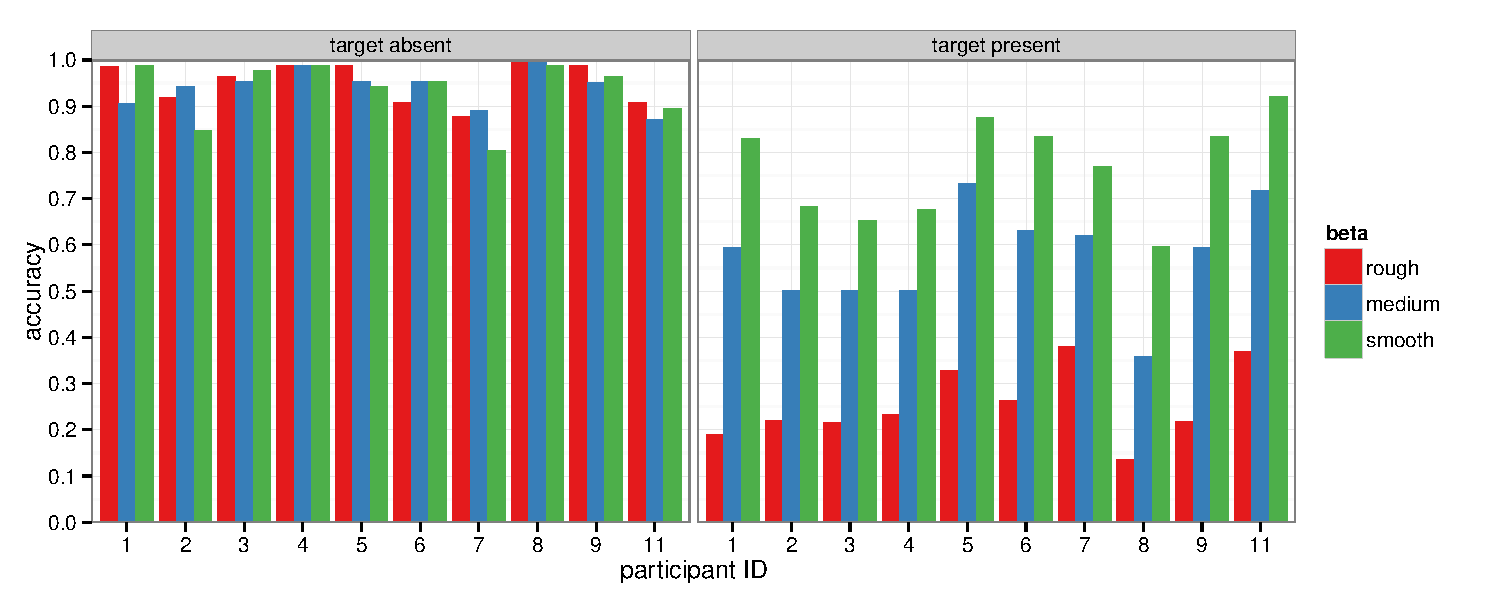
\includegraphics[width=8.5cm]{fig/targDet/targDetFalsePositive.pdf}
	\caption{Accuracy of responses to the target for each observer in the target detection study. We can see that the false positives rate is low.} 
	\label{fig:targDetFalsePositive}
\end{figure}

We analysed the results using a general linear mixed model (family=binomial), fit  with the model specified as $y\sim\beta*(x^2 + y^2)$, where $x$ and $y$ are the coordinates of the target. The model allowed for random slopes for $\beta$ as well as random intercepts. We find statistically significant effects ($p<0.001)$ of $\beta$ ($\chi^2(2)=3676$), $x^2$ ($\chi^2(1)=965$) and $y^2$ ($\chi^2(1)=1735$). The $\beta:x^2$ interaction was also significant ($\chi^2(2)=20.2$). A simplified version of the target detection function is showing in Figure \ref{fig:targDetEcc}.

\begin{figure}
	\centering
	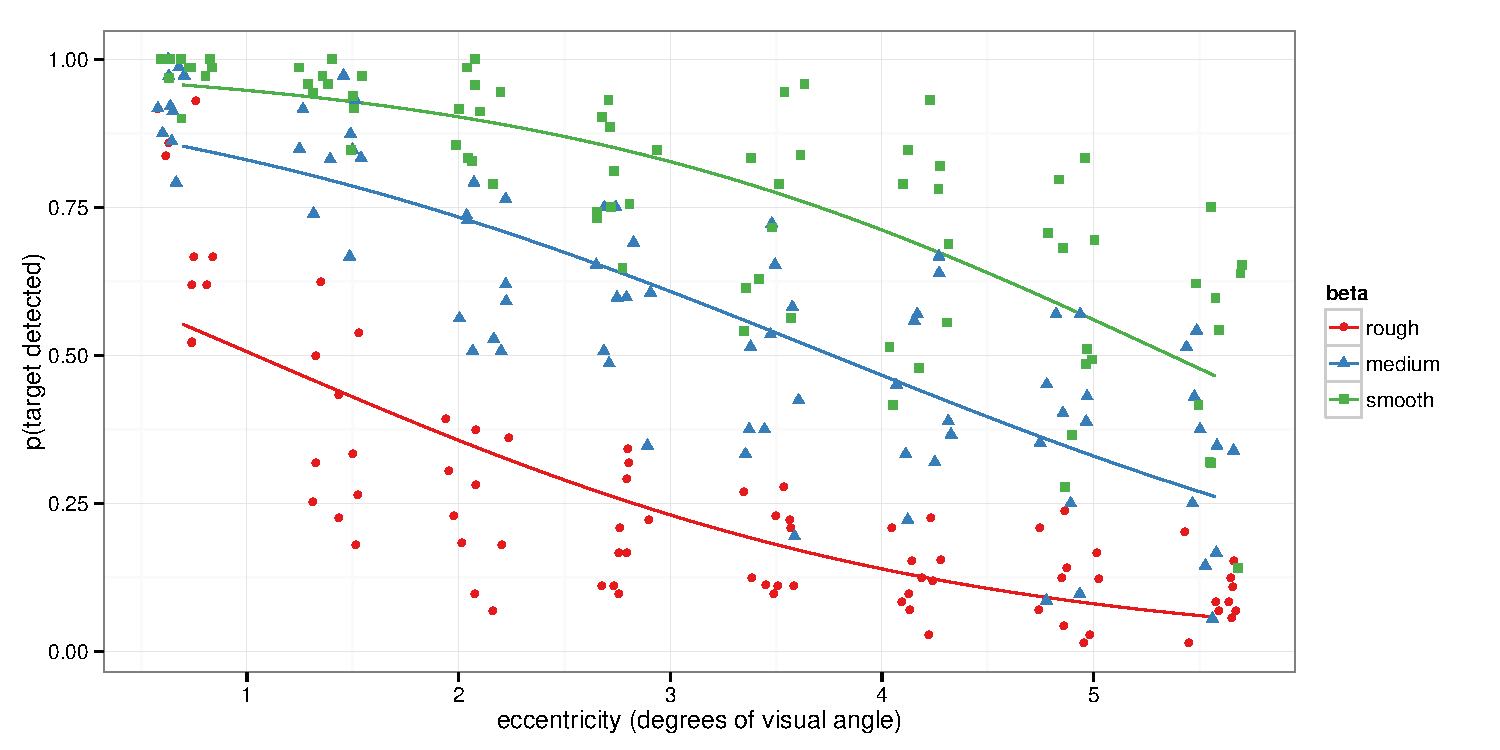
\includegraphics[width=8.5cm]{fig/targDet/targDetModelEccOnly.pdf}
	\caption{Probability of detecting the target, collapsed over angle (i.e., only taking the target's eccentricity into account). The individual points show each participant's performance, while the lines show a binomial fit (general linear model).} 
	\label{fig:targDetEcc}
\end{figure}

\subsubsection{Visual Search}
\label{sec:visSearch}

Mean accuracy was $99\%$ and $94\%$ for target present and absent trials respectively. We analyse log reaction time (RT) with a linear mixed model: $log(rt) \sim \beta +(\beta|\texttt{participantID})$. As expected, we find that $\beta$ has a statistically significant effect on log reaction times: $\chi^2=243.75$, $p<0.001$, with slower RTs to find targets on rougher surfaces. We also examined the spatial distribution of fixation locations using hotspot maps. As can be seen in Figure \ref{fig:hotspots}a, the observers exhibit a central bias \parencite{tatler2007} in their fixations locations, although there appear to be individual difference in the variance and spread of fixations. Importantly, the distinctive `doughnut' pattern of fixation locations observed in \textcite{najemnik-geisler2008} - and used as evidence that human observers are consistent with optimal search strategies - was not replicated. To explore whether this could be explained by the difference in the shape of the stimuli (we used square search areas which Najemnik and Geilser used circular areas). We tested this hypthesis by re-running the experiment with a subset of the participants using circular stimuli. As Figure \ref{fig:hotspots}b shows, this had no effect on the pattern of fixations.

\begin{figure}
	\centering
	\subfigure[square search areas.]{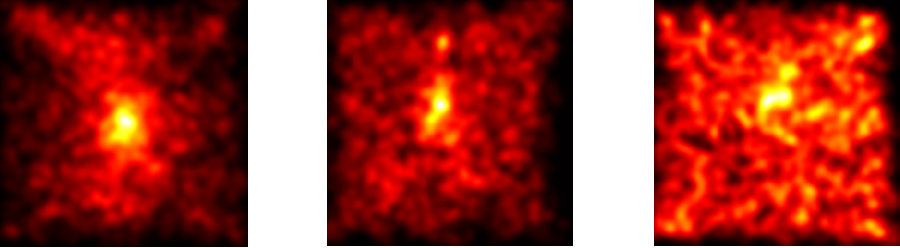
\includegraphics[width=8cm]{fig/visSearch/hotspotmaps.pdf}}
	\subfigure[circular search areas.]{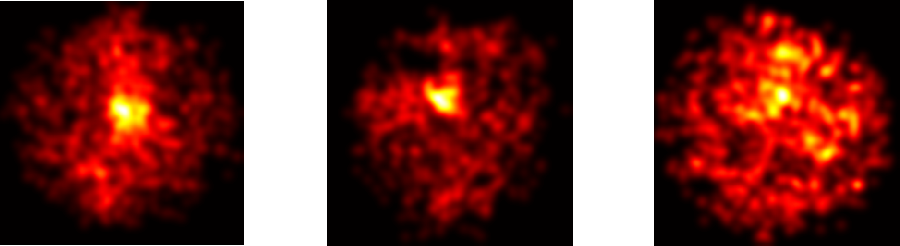
\includegraphics[width=8cm]{fig/hotspotmaps.pdf} }
	\caption{Hotspot maps for (a) square and (b) circular search areas for participants 2, 4 and 5 (left to right). We can see some individual differences, in particular, how strong the central bias is for each observer. However, there is no clear tendency to fixate above and below the fixation.} 
	\label{fig:hotspots}	
\end{figure}


%%%%%%%%%%%%%%%%%%%%%%%%%%%%%%%%%%%%%%%%%%%%%%%%%%%%%%%%%%%%%
\section{Search Strategies}
\label{sec:strats}
%%%%%%%%%%%%%%%%%%%%%%%%%%%%%%%%%%%%%%%%%%%%%%%%%%%%%%%%%%%%%

Here we describe a stochastic model of the search task described below, based on based on the visibility map. That is, the probability of detecting a target, $d$, located at $(x,y)$, when fixating $f_i = (x_f,y_f)$ is given by

\begin{equation}
 p(d_{x,y}|f_i,\beta) = F(\vec{b_1}\cdot\vec{\beta} + \vec{b_2}\vec{\beta} (x-x_f)^2 + \vec{b_2}\vec{\beta}(y-y_f)^2)
 \label{eq:targDet}
\end{equation} 

where $\vec{\beta}$ is a vector encoding the categorical factor $\beta \in \{\texttt{rough, medium, smooth}\}$ and $\vec{b_1},\vec{b_1},\vec{b_3}$ are the model's parameters to be fit.  $F$ is the logistic transform:

\begin{equation}
F(z)= \frac{1}{1+e^{-z}}
\end{equation}

This model is fitted to the results of the target detection experiment below, collapsing over participants. The coefficients are given in Table \ref{tab:targdetcoef} and this function is illustrated in Figure \ref{fig:targDet}.

\begin{figure}
	\centering
	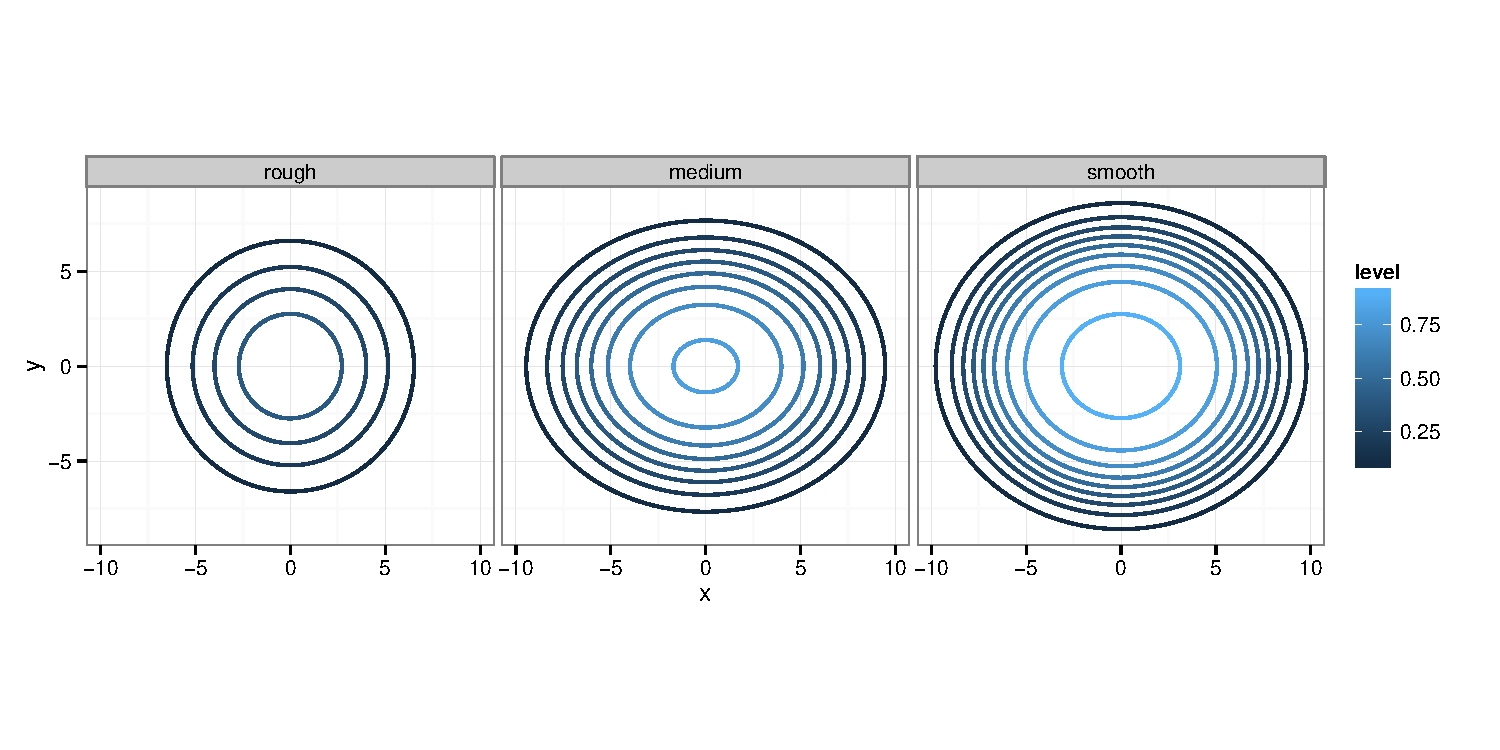
\includegraphics[width=8cm]{fig/targDet/aggtargdet2.pdf}
	\caption{Contour plot showing target detection model.} 
	\label{fig:targDet}
\end{figure}

\begin{table}
\centering
\begin{tabular}{c|ccc}
 $\beta$ 	& rough & medium & smooth \\
\hline
intercept	& -0.17 & 1.27 & 2.39\\
$x^2$	& -0.089 & -0.062 & -0.074 \\
$y^2$	& -0.103 & -0.103 & -0.103 \\
\end{tabular}
\caption{Coefficients used in Equation \ref{eq:targDet}, the target detection function.}
\label{tab:targdetcoef}
\end{table}


The main aim of this study is to explore the extent to which visual search performance can be explained by a random walk. For each fixation, the stochastic searcher uses the target detection function given in Equation \ref{eq:targDet} to determine if the target is present. To decide where to fixate next, this model samples a saccade at random (from empirical data), conditioned on the current fixation location, $S(x',y',x_i, y_i)=p\left((x',y')|(x_i,y_i)\right)$. We base $S$ on the distribution of saccades recorded during the visual search experiment. To estimate $S$, we start by quantising the fixations to a $Q\times Q$ grid ($Q=32$). Then we simply count the number of saccades from $(q_{x_1}, p_{y_1})$ to $(q_{x_2}, p_{y_2})$, $1\leq x_i, y_i \leq Q$. As the last saccade in each trial is likely to be directed towards the target, rather than searching for the target, these saccades are not included in this distribution. We then convolve $S$ with a four-dimensional Gaussian filter ($\sigma=3$). Figure \ref{fig:saccDistExample} shows a simplified version of this distribution (with $Q=3$). 

\begin{figure}
	\centering
	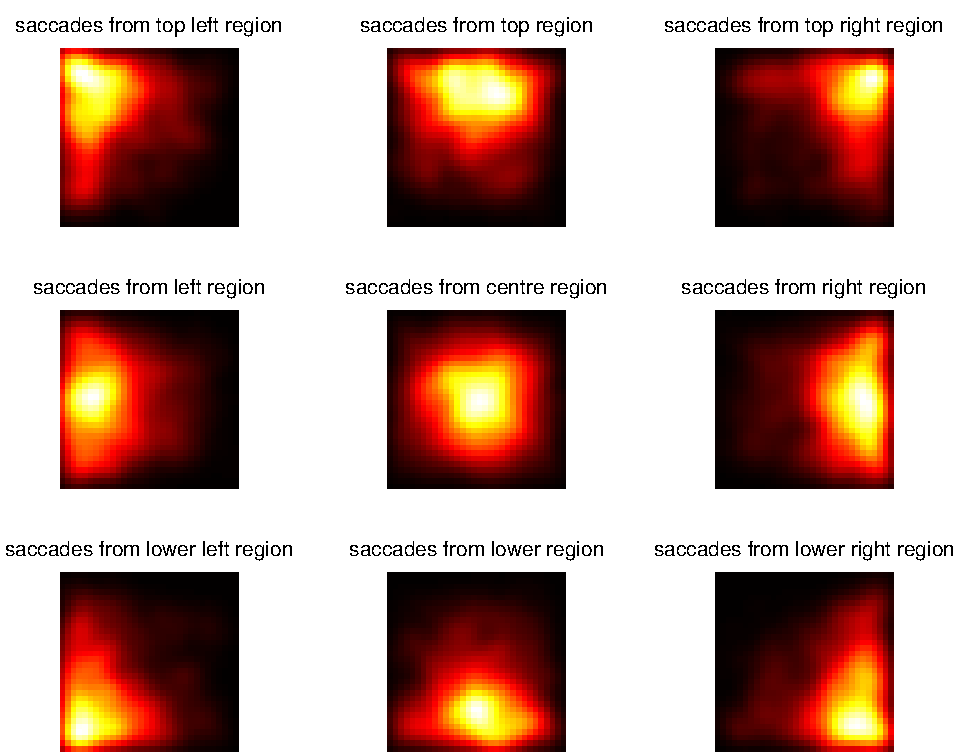
\includegraphics[width=8cm]{fig/saccDistExample.pdf}
	\caption{Each subplot shows a hotspot map of fixation locations from a different region of the stimuli. For example, we can see that saccades originating from the corner regions tend to be directed back towards the centre, or along one of the edges.}
	\label{fig:saccDistExample}
\end{figure}

The use of this distribution allows the stochastic searcher to act as a realistic baseline: it will make saccades with amplitudes and directions similar to those made by human observers, and it avoids making saccades to locations outside of the search area. On the other hand, as the probability of making a fixation to a given location is only conditioned on the sample of saccades to that region in previous data, it has no memory of where it has looked before, and it has no notion of inhibition of return or saccadic momentum. Furthermore, the stochastic searcher does not adjust its behaviour based on the difficulty of the search task or the probability of detecting the target. 


% \subsection{Optimal searcher}

% The optimal model uses the target detection function, $p(d_{x,y}|f_i,\beta)$, to estimate $p(t_{x,y})$, the probability that the target is located at $(x,y)$, defined as:

% \begin{equation}
% P_i(x,y) = p(t_{x,y} | \beta, f_1,\ldots, f_i)
% \end{equation}

% \subsubsection{Probability that target is located at $(x,y)$}

% We start off by setting $P_0$ to our prior on where the target is likely to be located. We will use a uniform distribution over the search area: $P_0(x,y) \propto \hat{P_0}=1$. (i.e.,  $P_0(x,y) = \frac{1}{N^2}$, where $N^2$ gives the area of the search stimulus). However, $P_0$ could be set to any arbitrary distribution. 

% After each fixation, we use Equation \ref{eq:targDet} to check if the target has been detected. If the target is detected then $P_i = 1$ at the target's location, 0 everywhere else and the search process is terminated. If the target is not detected then, assuming (i) perfect memory and (ii) that $p(d_{x,y} | \beta, f_i)$ $\forall i$ are independent, we define $P_i\propto \hat{P_i}$ as: 

% \begin{align}
% P_i(x,y) \propto \hat{P}_i(x,y)	&= p(t_{x,y} | \beta, f_1,\ldots, f_i)\\
%  							&= p(t_{x,y} | \beta, f_1,\ldots, f_{i-1})\times p(t_{x,y} | \beta, f_i)\\
%  							&= \hat{P}_{i-1}(x,y)\times (p(\neg d_{x,y} | \beta, f_i))
%  			\label{eq:Pupdaterule}
% \end{align}

% The logic of this is as follows. Consider our first fixation $f_1 = (x_1,y_1)$, a potential target location $(x',y')$ close to the current fixation, and let us assume that we have not yet detected the target. If the target was located at $(x',y')$, then we would have a relatively good chance of detecting it. For the purpose of this explanation, let us assume that $p(d_{x',y'}|f_1)=0.8$, that is, if we fixate at $(x_1,y_1)$ then we have a $80\%$ chance of detecting the target if it is located at $(x',y')$. Now let us consider the probability that the target is indeed located at $(x',y')$. If there were an $80\%$ chance of target detection, but no target was detected, there is (up to a normalisation step to take into account the total number of possible target locations) a $20\%$ chance that the target is located at $(x',y')$. More generally:
% \begin{equation}
% p(t_{x',y'}|f_1) \propto p(\neg d_{x',y'}|f_1)
% \end{equation}
% We can iterate over successive fixations using Equation \ref{eq:Pupdaterule}.

% \subsubsection{Choosing where to fixate next}

% Once we have calculated $\hat{P}_i$ we use it to select the next fixation location. As we are only calculating $P_i$ up to a normalisation constant, the map that we actually calculate, $\hat{P_i} =  \hat{P}_{i-1}(x,y)\times p(\neg d_{x,y} | \beta, f_i)$, has the property that $\hat{P}_i(x,y)\leq\hat{P}_{i-1}(x,y)$ $\forall i,x,y$. This can be thought of as measuring how much we still have to search different regions of the stimulus. Our model will make a fixation at the point $f_{i+1}=(x_{i+1},y_{i+1})$ that maximises the difference between $P_i$ and $P_{i+1}$. This can be expressed as: 

% \begin{equation}
% (x_{i+1},y_{i+1}) = \argmin_{f_j=(x_j,y_j)}\sum_{x,y} P_i(x,y)p(\neg d_{x,y}|\beta, f_j)
% \end{equation}

% This process is illustrated in Figure \ref{fig:planningFix}. In order to reduce computation time, the simulation takes place at a lower resolution, with $N=256$ rather than 1024.


% \begin{figure}[tb]
% 	\begin{center}
% 		\subfigure[fixation 1]{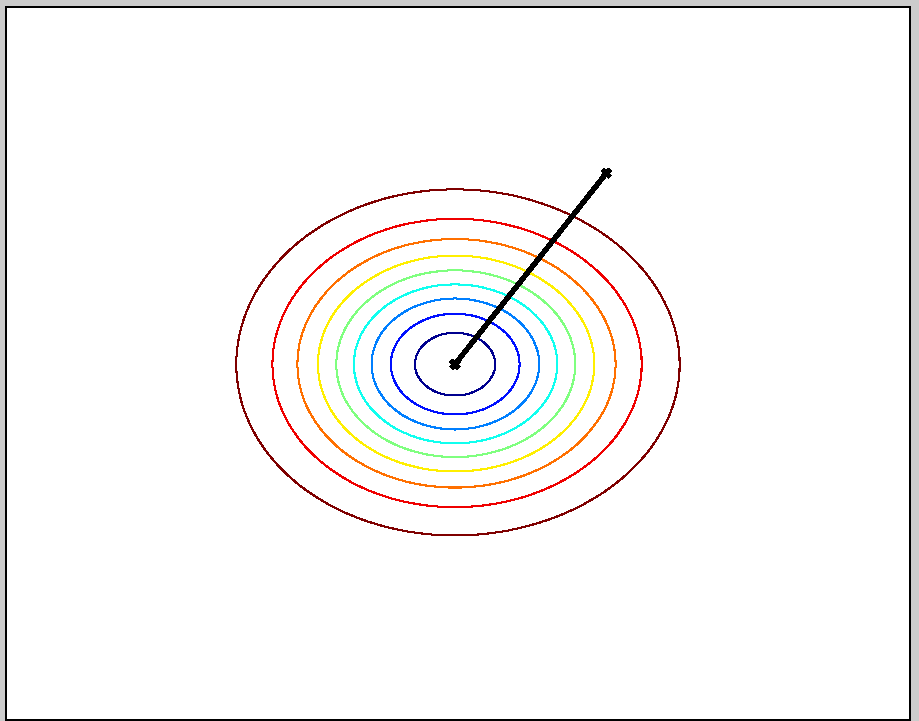
\includegraphics[width=3cm]{fig/fixplanning/fixation1.pdf}}
% 		\subfigure[fixation 2]{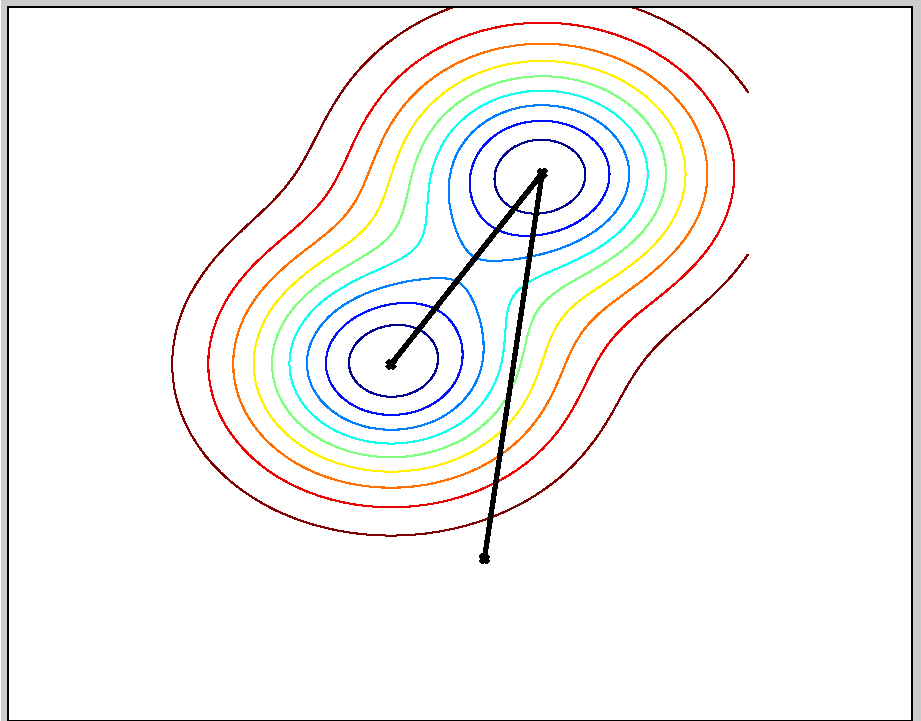
\includegraphics[width=3cm]{fig/fixplanning/fixation2.pdf}}
% 		\subfigure[fixation 5]{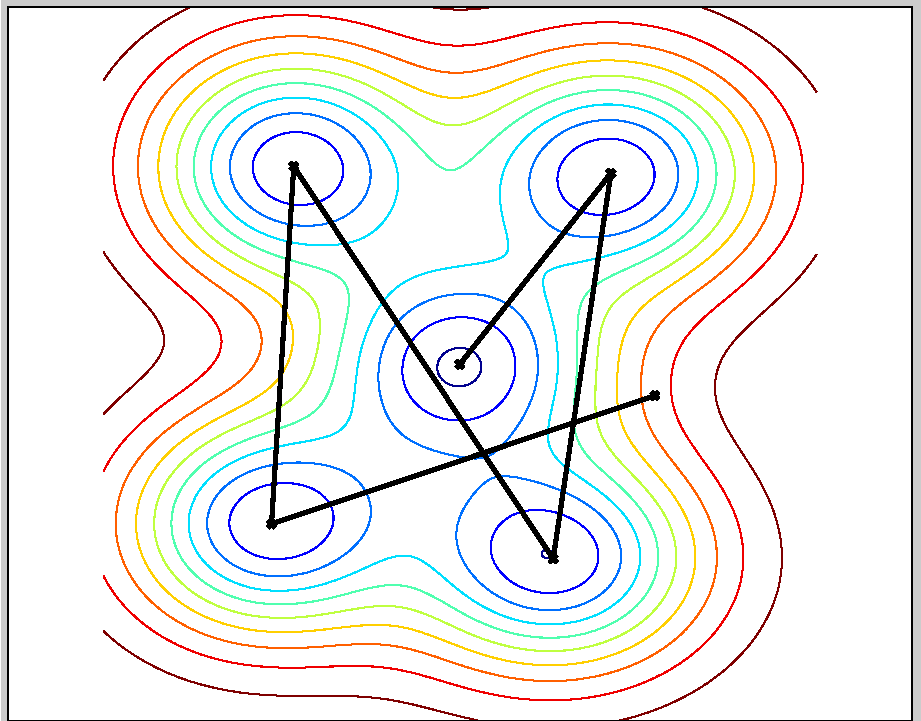
\includegraphics[width=3cm]{fig/fixplanning/fixation5.pdf}}
% 		%\subfigure[fix 10 $\beta=1.6$]{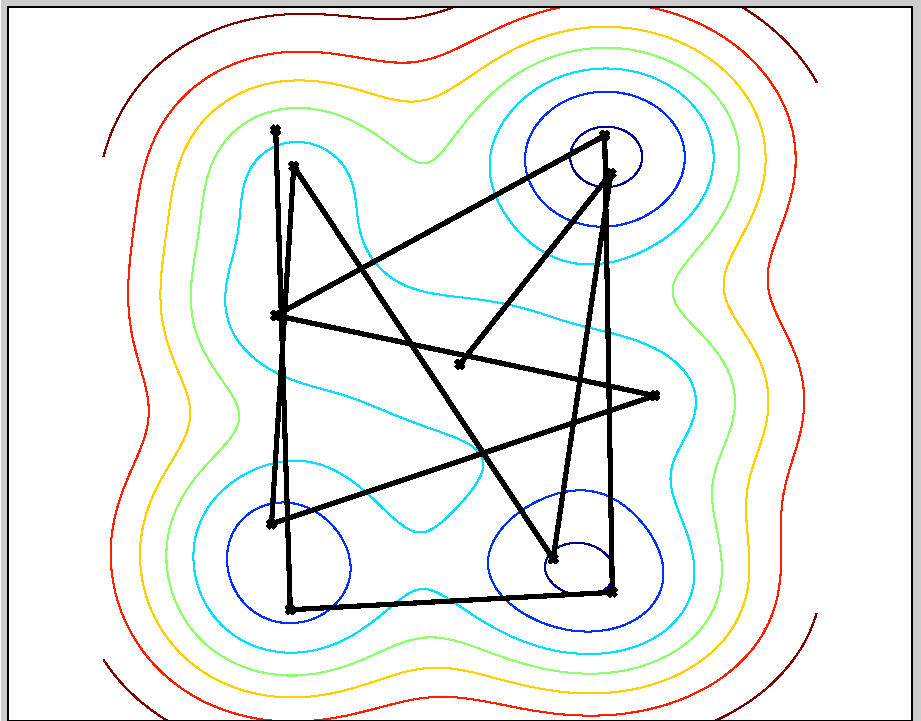
\includegraphics[width=3cm]{fig/fixplanning/fixation10.pdf}}
% 		\subfigure[fixation 1]{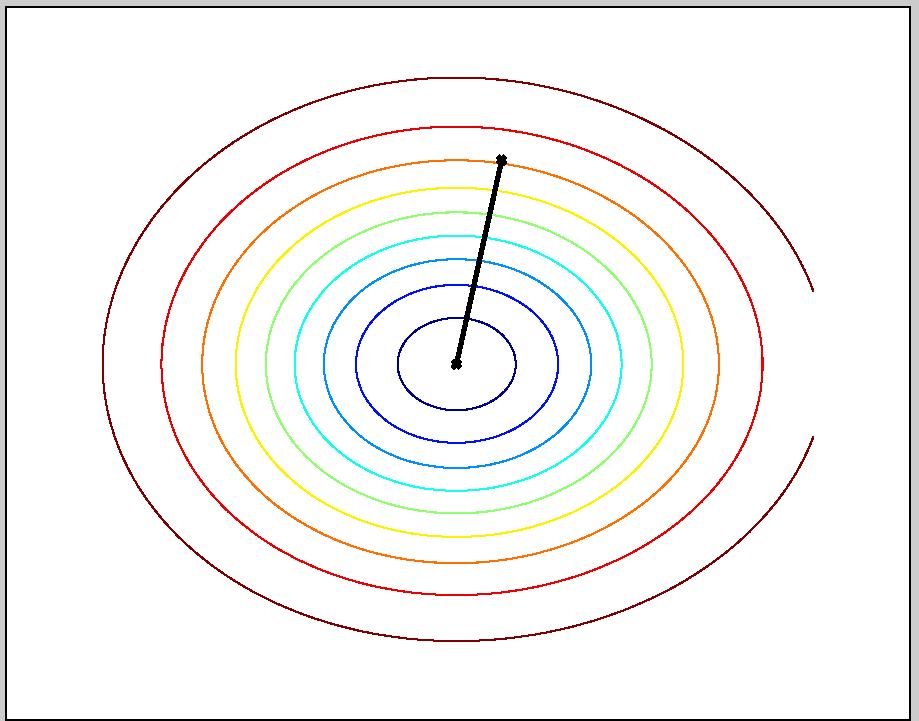
\includegraphics[width=3cm]{fig/fixplanning/fixation1-2.pdf}}
% 		\subfigure[fixation 2]{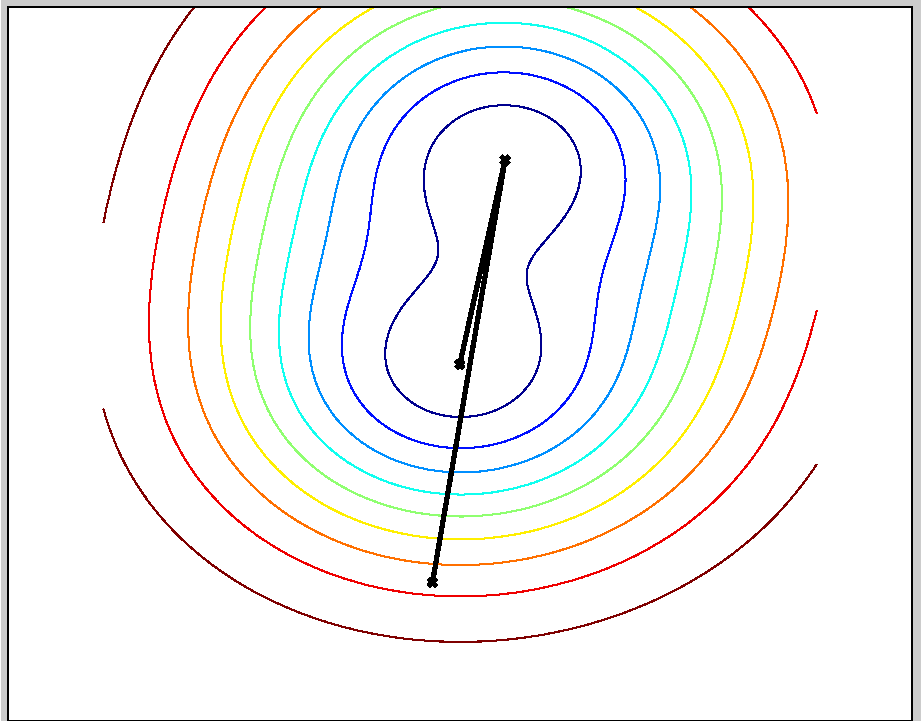
\includegraphics[width=3cm]{fig/fixplanning/fixation2-2.pdf}}
% 		\subfigure[fixation 5]{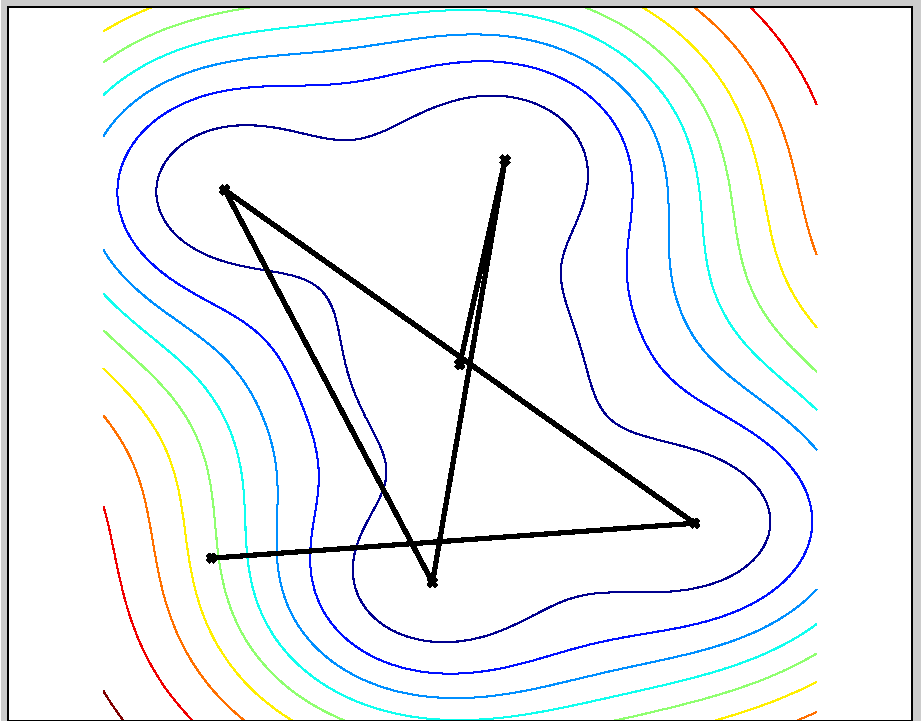
\includegraphics[width=3cm]{fig/fixplanning/fixation5-2.pdf}}
% 		%\subfigure[fix 10 $\beta=1.7$]{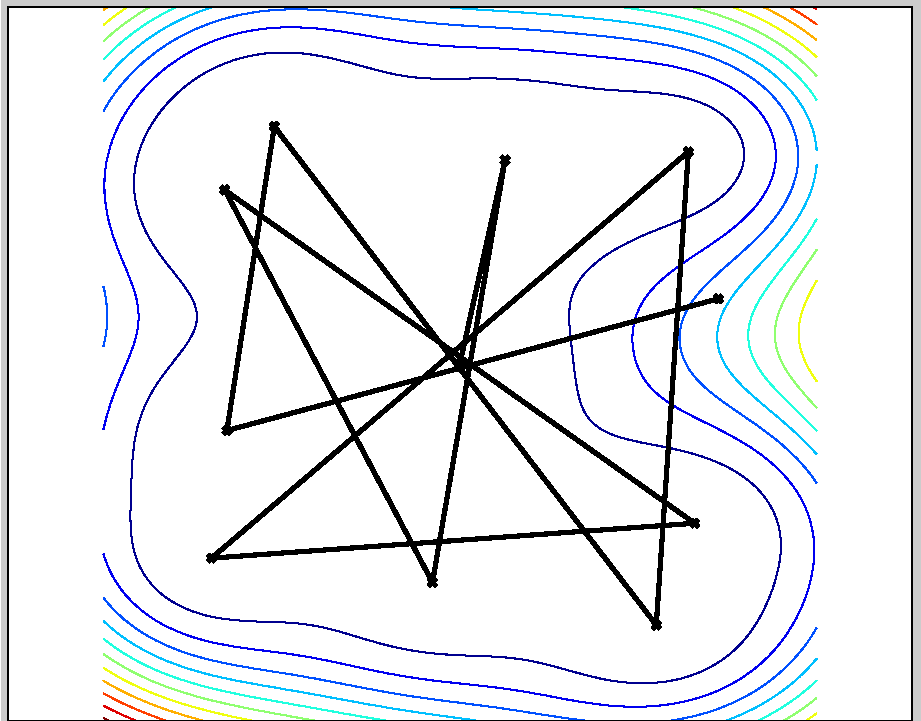
\includegraphics[width=3cm]{fig/fixplanning/fixation10-2.pdf}}		
% 	\end{center}
% 	\caption{This figure shows how $P_i$ is updated with each fixation and used to plan the next fixation. (a), (b) and (c) show fixation 1,2, and 5 in the hard condition, while (d), (e) and (f) show how search progresses in the easy condition.}
% 	\label{fig:planningFix}
% \end{figure}


\subsection{Comparison between human observers and the model}

We now compare the model to human performance by simulating search over the same number as trials used in the human experiment. As we can see from Figure \ref{fig:numFixHumanModel}, the stochastic searcher requires a similar number of fixations to find the target as our human participants. We can analyse how the number of fixations differs between human and stochastic observers using a general linear mixed effect model (family="poisson"), with random slopes for $\beta$ and random intercept: $n_{fix} \sim \beta * s + (1+\beta | p_h)$, where $s$ is a two-level factor coding human/model and $p_h$ is the human observer id. The only statistically significant difference between the human observers and the stochastic model was for the smooth surfaces, for which the stochastic search model required on average half a fixation more than the human observers in order to find the target. 

\begin{figure}
	\centering
	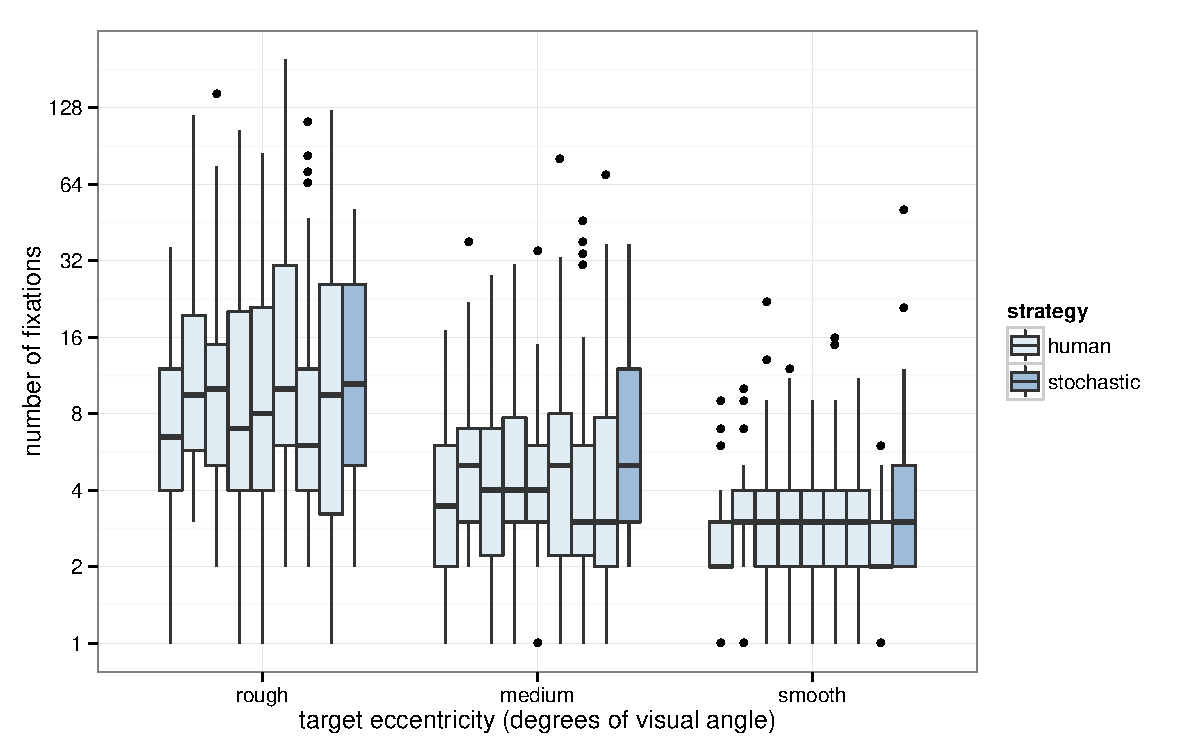
\includegraphics[width=8.5cm]{fig/modelComp/numFixHumanModel.pdf}
	\caption{Number of saccades made by human observers and the stochastic search simulation.} 
	\label{fig:numFixHumanModel}
\end{figure}

%We can also look at the saccade statistics to see if they offer a way to distinguish between the two models and determine which offers the more human-like behaviour. Figure \ref{fig:exScanpaths} shows some example scanpaths. We can see that the optimal model favours making fixations in the centres of the four quadrants of the search area. These points maximise the area of the stimulus in the effective field of view while minimising the overlap with earlier fixations made to other regions. While this involves re-fixating a previously fixated location, given the low probability of detection on rough surfaces (Figure \ref{fig:targDetEcc}), this is not as unintuitive as it may initially appear - there is a $50\%$ chance that the model will miss a target at fixation on a rough surface. We can also see that after fixating the centre of each quadrant three times (giving a probability $p \approx 1-0.5^3 = 0.875$ of detecting the target at these points), the model switches to fixate the in-between regions. 

Figure \ref{fig:onetwostats} shows the distribution of saccade amplitudes and directions. Interestingly we see that even though the stochastic model is only constrained by the distribution of saccades made by human observers, this is sufficient to give a reasonable match for the displacement over two saccades, and hence it exhibits a similar level of inhibition of return as the human observers. The largest difference between the model and the observers can be seen in the relative direction between two successive saccades. Human observers show a large peak around $0^{\circ}=360^{\circ}$ which indicates saccadic momentum: a second saccade is likely to be made in the same direction as the first saccade. 

% \begin{figure}
% 	\centering
% 	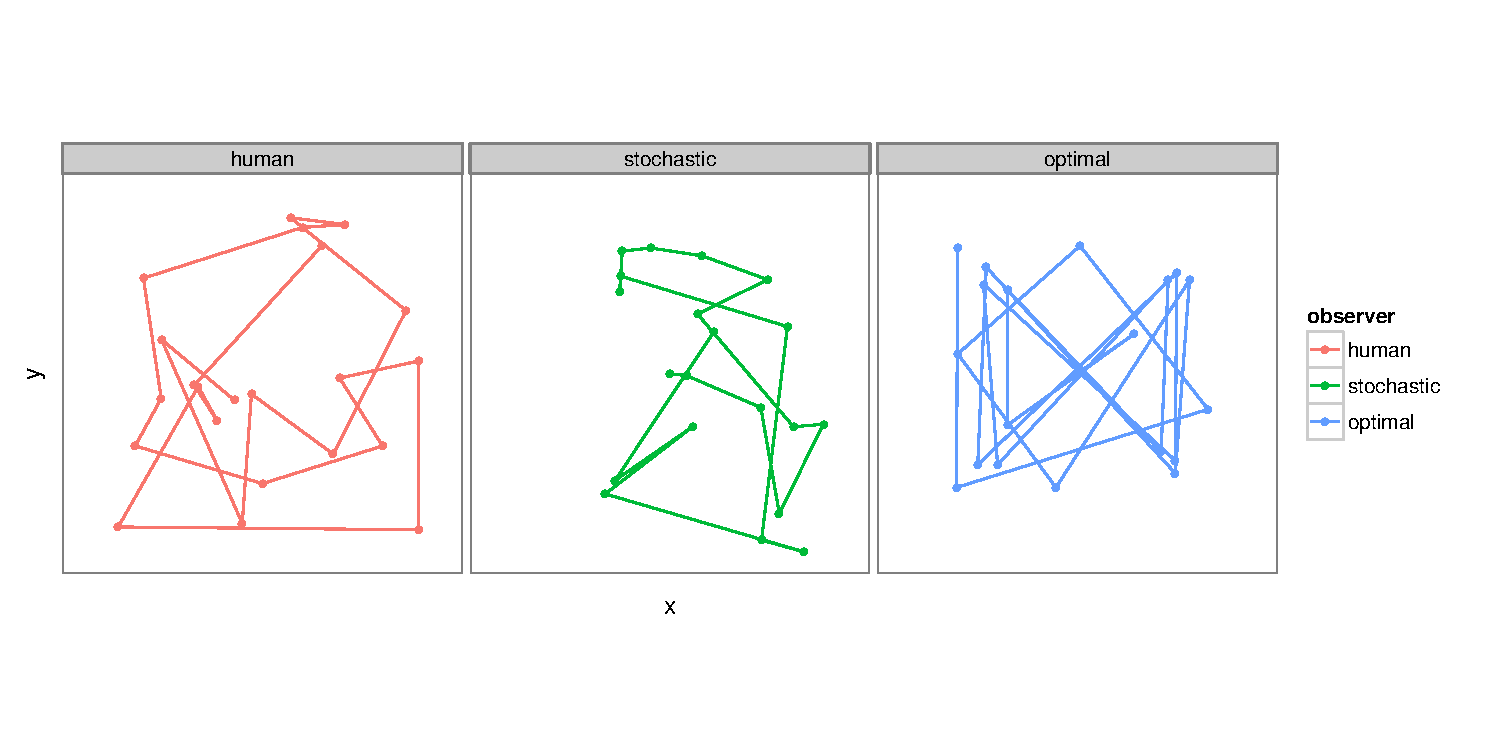
\includegraphics[width=8cm]{fig/modelComp/exScanpaths.pdf}
% 	\caption{Example scanpaths made by a human, stochastic and optimal observer for a rough surface. We can see that similarly to \textcite{najemnik-geisler2008}, the optimal model shows a preference for several fixed points on the stimulus. These are the locations which maximise the information gained via para-foveal vision, and minimise the proportion of the effective field of vision that falls outside of the search area. The centre is avoided after the initial fixation because it is frequently sampled by peripheral vision.} 
% 	\label{fig:exScanpaths}
% \end{figure}


\begin{figure}
	\centering
	\subfigure[]{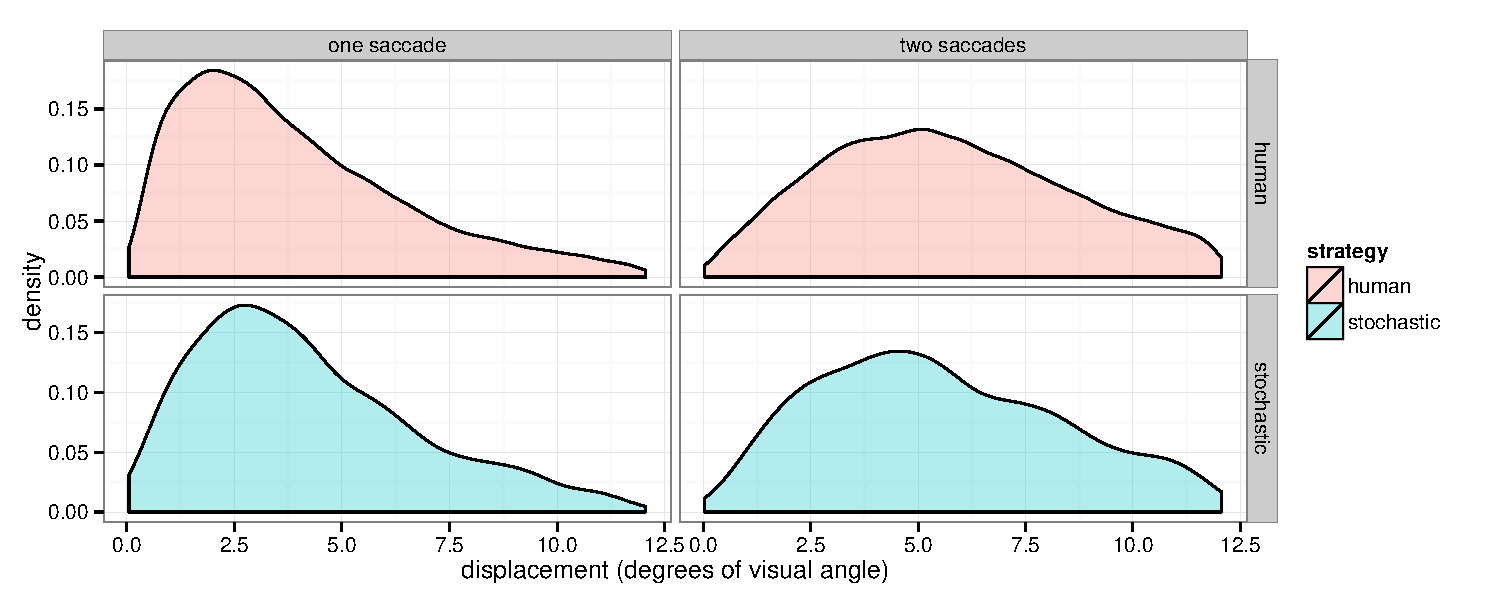
\includegraphics[width=8cm]{fig/modelComp/onetwosaccamp.pdf}}
	\subfigure[]{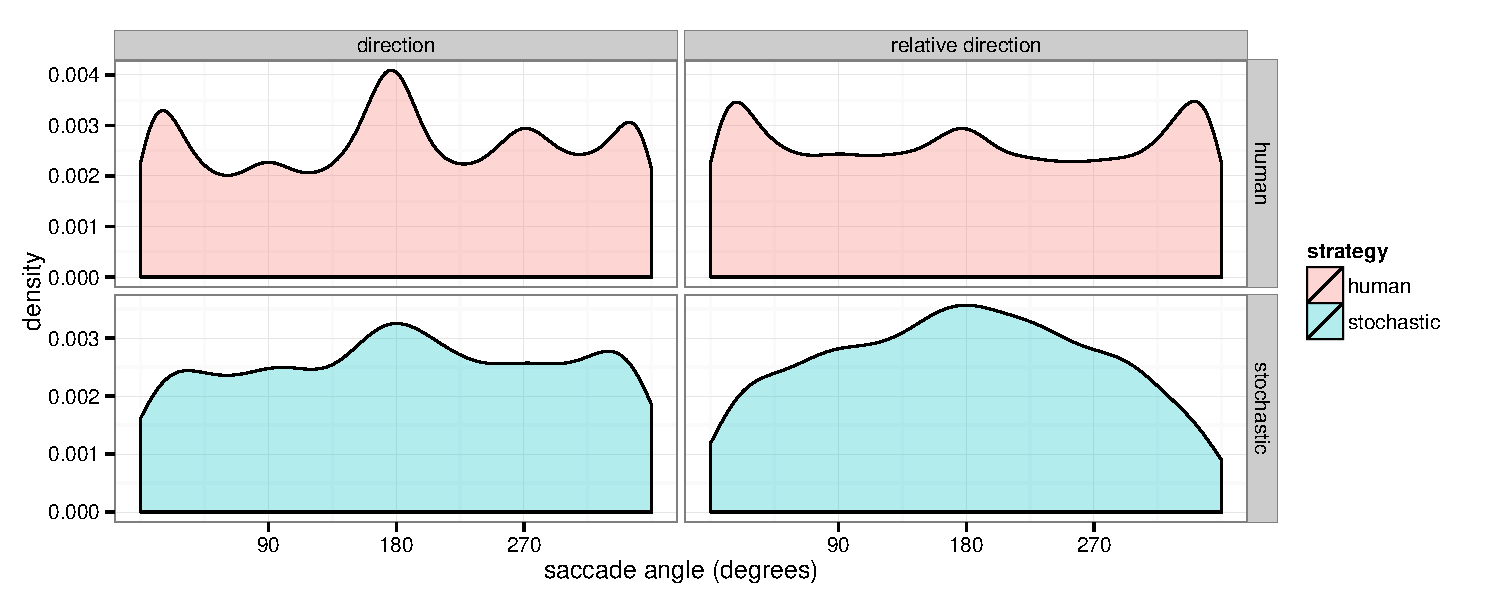
\includegraphics[width=8cm]{fig/modelComp/saccAngles.pdf}}
	\caption{(a) Displacement over one and two saccades. (b) Absolute and relative direction of saccades. The fact that the stochastic model matches the distribution of displacement and direction over a single saccade is a direct result of sampling from empirical data and is therefore unsurprising.}
	\label{fig:onetwostats}
\end{figure}

\subsection{Discussion}

In general, the stochastic model results provide a good match for human behaviour, in terms of the number of fixations to find the target. This conclusion is somewhat surprising given that \textcite{najemnik-geisler2008} demonstrated that the number of fixations required by observers to find a target is also consistent with an optimal strategy. Najemnik and Geilser also pointed to the distribution of fixation locations as evidence that humans employ an optimal strategy: the model predicts a distribution with peaks above and below the central fixation cross, which they also observed in their three human searchers.  However, using a larger sample of participants, we found that this result did not replicate. One plausible reason our results from nine observers did not produce this pattern is that our experiments used a square search array while their array was circular. In order to investigate this potential reason for the discrepant findings, we repeated our visual search experiment with a circular search array with three of our observers, and found that this made no difference. 

%%%%%%%%%%%%%%%%%%%%%%%%%%%%%%%%%%%%%%%%%%%%%%%%%%%%%%%%%%%%%
\section{Reanalysis of \textcite{clarke2009}}
\label{sec:surfacesearch}
%%%%%%%%%%%%%%%%%%%%%%%%%%%%%%%%%%%%%%%%%%%%%%%%%%%%%%%%%%%%%

In the previous experiment we found evidence that a random walk is a viable explanation of human visual search performance. In this section we apply the same analysis to a similar dataset \parencite{clarke2009}. The empirical data were collected in a different lab with a different eye-tracker and fixation filter, and should therefore provide a good test of the robustness of our results. In addition, in the visual search task used in this dataset the target's eccentricity is systematically varied, allowing us to compare the stochastic model to human performance separately for different target eccentricities. As in Experiment 1, we first generated a target visibility function using a target detection task. We collected target visibility data from two naive observers who did not perform the visual search task.

%%%%%%%%%%%%%%%%%%%%%%%%%%%%%%%%%%%%%%%%%%%%%%%%%%%%%%%%%%%%%
\subsection{Target detection experiment}

%%%%%%%%%%%%%%%%%%%%%%%%%%%%%%%%%%%%%%%%%%%%%%%%%%%%%%%%%%%%%

\subsubsection{Observers}

Two observers carried out all the trials, split into twenty blocks of 132 trials each, over a number of days. They were paid \pounds50 each. The research was conducted in accord with the Code of Ethics of the World Medical Association (Declaration of Helsinki) and informed consent was obtained from both observers. 

\subsubsection{Stimuli}

Surface textures were created as detailed in Experiment 1. For the target present trials, the target was located at one of 72 potential locations: nine different eccentricities were used ($0.84^{\circ}\leq r\leq 7.5^{\circ}$), and eight evenly-spaced orientations. For each parameter combination, 20 different trials were created.  Based on pilot results, we created 160 target absent trials for each value of $\beta$, giving a total of 2160 target present trials and 480 target absent trials. This ratio of target present to absent trials ensured that observers made roughly equal numbers of ``present'' and ``absent'' responses.

\subsubsection{Set-up}

Observers were instructed to keep their eyes fixated on the centre of the image. After each trial, they were asked to respond with a button press to indicate if they had seen the target or not.  Each trial consisted of a fixation cross (500ms), stimulus (200ms), white noise mask (500ms), and finally a fixation cross was displayed until a target present or absent response was given. Trials were presented in a random order. 
\par
A Tobii x50 eyetracker was used to sample the observers' gaze every 20ms and trials were included in the further analysis only if (i) the mean gaze location was within $1^{\circ}$ of the central fixation cross (ii) the standard deviation of the gaze's $x$ and $y$ components was less than $2/3^{\circ}$.

\subsubsection{Results}

$13.6\%$ of trials were removed from analysis (due to breaking central fixation). 
We first checked the false positive rate on target absent trials, which were similar to those seen in Experiment 1 (less than $10\%$ in all conditions for both observers). We therefore focus on the probability of detecting the target when it was present as a measure of visibility. We collapse over the two observers and fit a model as in Experiment 1. Results and model coefficients are similar. 

\subsection{Visual Search Dataset}

The visual search data were taken from an experiment originally published in \textcite{clarke2009}. The methods and data are summarised here. 

\subsubsection{Observers}
Seven observers, aged 18-30, were given several practice trials and were informed that the target would be present in all trials and would always be an indent in the surface of the same size and shape. They were instructed to respond by pressing the space bar on the keyboard once they had found the target. No time limit was imposed on the task. Observers were told to inform the experimenter if they were having great difficulty in finding the target, in which case they were allowed to skip the trial (in practice this accounted for less than 1\% of trials). 

\subsubsection{Surface Stimuli}
This stimuli were created as in Experiment 1. For each trial a target was positioned randomly on a circle, centred on the middle of the image, with radius $1.7^{\circ} \pm 0.7^{\circ}$, $3.8^{\circ} \pm 0.7^{\circ}$ or $5.9^{\circ} \pm 0.7^{\circ}$ visual angle. 

\subsubsection{Set-up}
Stimulus presentation was controlled by Clearview (Tobii Technology Inc). All stimuli were $1024 \times 1024$ pixels in size and displayed on a NEC LCD2090UXi monitor. The pixel dimensions were 0.255mm by 0.255mm resulting in images with physical dimensions 26.1cm by 26.1cm. The monitor was linearly calibrated with a Gretag-MacBeth Eye-One; maximum luminance was set at 120 cd/m$^2$. This results in the rendered images appearing as if they were under bright room lighting conditions.

A Tobii x50 eye-tracker was used to record observers' gaze patterns. The fixation filter was set to count only those fixations lasting longer than 100 ms within an area of 30 pixels. The accuracy of the eye-tracker was $0.5^{\circ}$ to $–0.7^{\circ}$ and the spatial resolution was $0.35^{\circ}$. The viewing distance was controlled by use of a chin rest placed 87cm away from the display monitor. At this distance, one pixel is approximately 1 arcminute of visual angle; images subtend $16.7^{\circ}$ and the targets subtend $0.66^{\circ}$ of visual angle. 

\subsubsection{Results}
\label{sec:SearchPerf}
The number of fixations required to find the target is shown in Figure \ref{fig:numFixHumanModelClarke2009}. Using a generalised linear mixed model  (\texttt{family="poisson"}) we confirm that both roughness ($\beta$) and target eccentricity, along with their interaction, have a statistically significant effect ($p<0.05$) on the number of fixations required to detect the target. 

\subsection{Comparison with Search Models}

We now compare the model to human performance by simulating search over the same number as trials as used in the original experiment (incorrect and target absent trials are discarded). The results closely match those of Experiment 1. In terms of the number of saccades required to find the target, we find the stochastic searcher offers very similar performance to the seven human observers over the range of surface roughness's and target eccentricities used (Figure  \ref{fig:numFixHumanModelClarke2009}).

\begin{figure}
	\centering
	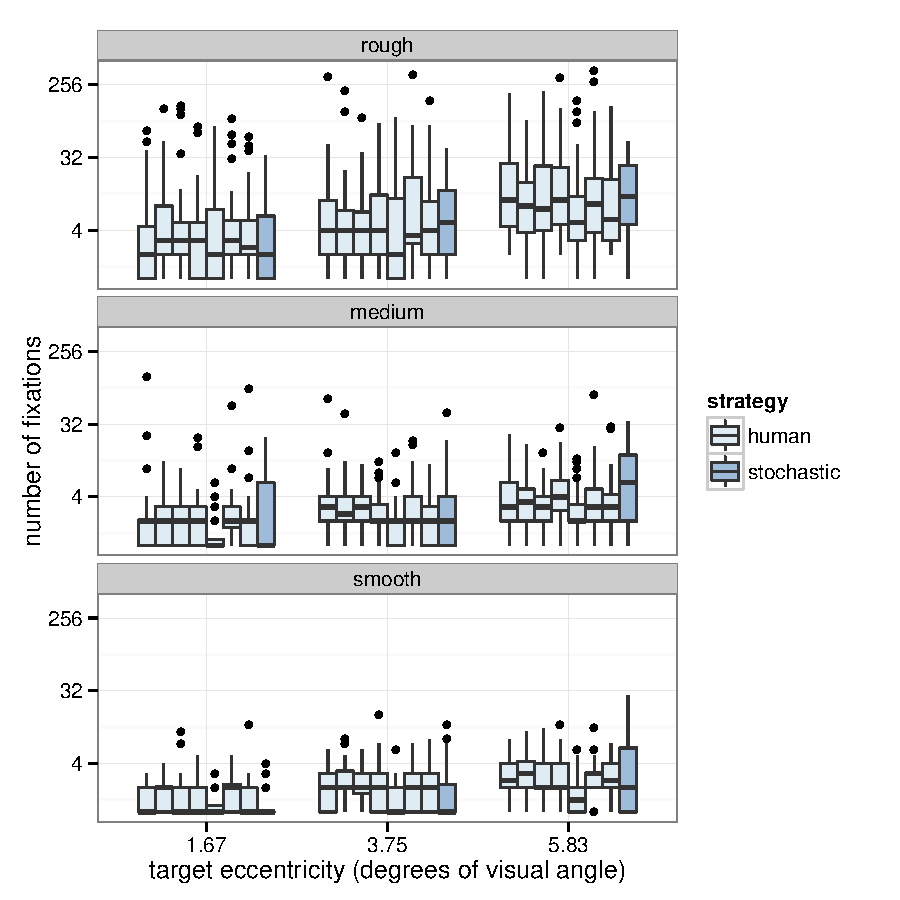
\includegraphics[width=8.5cm]{fig/numFixHumanModelclarke2009.pdf}
	\caption{Number of saccades made by human observers and search simulations. We can see that the stochastic search model is sufficient to explain the number of fixations required to find the target.} 
	\label{fig:numFixHumanModelClarke2009}
\end{figure}


%%%%%%%%%%%%%%%%%%%%%%%%%%%%%%%%
\section{General Discussion}
%%%%%%%%%%%%%%%%%%%%%%%%%%%%%%%%

Human visual search performance can be modelled by a stochastic process. Beyond the number of fixations required to find the target, the stochastic model also does a reasonable job of explaining the spatial distribution of fixations, the frequency of saccade amplitudes, and the relative angles of sequences of saccades. 

It is interesting that the stochastic and optimal models -- two models that have very different architectures and produce very different search behaviour -- could both take a similar number of fixations as humans to detect a target. Clearly there is more than one way to achieve this single end, and maximising the probability of detecting the target separately for each fixation is not a requirement for relatively efficient search to be achieved. It should be mentioned that  \textcite{najemnik-geisler2005} did compare their optimal model to a random baseline, and that this baseline made far more fixations to detect the target than either the optimal model or human searchers. However, their random model selected uniformly random coordinates within the search stimulus as the target of each fixation in the sequence. This baseline differs from the current model in that it does not take into account the natural tendencies in saccade behaviour that make some fixations and sequences of fixations more likely than others. Our results demonstrate that these tendencies alone, irrespective of any knowledge about previous fixations or target detection probabilities, can produce efficient search. 


\par

An important difference between our study and \textcite{najemnik-geisler2005, najemnik-geisler2008} is in the experiment used to collect data to create the
target visibility map. \textcite{najemnik-geisler2005, najemnik-geisler2008} made
use of a 2AFC procedure in which observers had to select which of two
intervals contained the target. Target location was blocked and observers were
also spatially cued to the target location on each trial. Cueing a target's
location has long been known to improve performance \parencite{posner1980},
specifically by enhancing the target signal \parencite{yeshurun1998}. Indeed, our pilot experiment comparing these two measures of sensitivity demonstrated that the 2AFC method inflates sensitivity, particularly in the difficult search conditions, and reduces differences between difficulty manipulations. We therefore
opted to use a simpler target detection procedure in which the observer did
not know the target's location ahead of time. We chose this because it is a
better approximation of visual sensitivity in the context of visual search,
where the target location is also not known. Another key difference is that \textcite{najemnik-geisler2008} report a
tendency to fixate above and below the centre of the search display for both
humans observers and their optimal model. This tendency did not appear in our
human data, even when we re-ran the search experiment using a circular search
display to match the one used in \textcite{najemnik-geisler2008}.  

\par 

We do not wish to claim that stochastic selection of saccades is the only process
involved in search. As stated in the introduction, search strategy and feature
extraction work together to produce search behaviour. A stochastic process
would work in concert with guided search in a more typical search context in
which there are many objects and/or contextual information available. One
could imagine that if there are several search items that could potentially be
the target, a random walk model could be used to choose which item should be
fixated next. Also, although our model did not need any form of memory or
inhibition of return to achieve human-like behaviour, we do not mean to
suggest there is no inhibition of return in human search. Indeed, as our
stimuli contain no search objects, any IOR processes would have to be
operating in spatiotopic coordinates defined with respect to stimulus
boundaries, rather than being applied to discrete search objects. IOR is
strengthened by objects \parencite{jordan1998}, and this may be particularly true
when the eyes move, necessitating inhibition of spatiotopic, rather than
retinal, coordinates (e.g., \textcite{kruger2013}).

\par

Our results suggest that the process of deciding where to look next may be driven by a simple random selection from a subset of possible saccades. What determines this subset of possible saccade is an interesting question, but is likely to involve a combination of visual and motor constraints together with a lifetime of experience searching for objects. The mechanism that has been assumed to subserve efficient eye movement behaviour in natural tasks is reinforcement learning (e.g. \textcite{hayhoe2014}). Prior learning during search tasks could cause particularly effective saccades and sequences of saccades to be selected rapidly and efficiently, without the need for a computationally taxing process of keeping track of the probability of a target being in any possible location given target visibility and a memory of all previous fixations over an extended sequence. Our conclusion is consistent with recent work suggesting humans are sub-optimal in search (\textcite{morvan2012, verghese2012, zhang2012}), in that saccades during search do not appear to maximise the probability of detecting the target based on previous fixations and knowledge about the limits of our own visual acuity. Fortunately, our results suggest this kind of optimality is not a pre-requisite for search efficiency: A stochastic model based on human saccade data can perform as well as an optimal model.

\section*{Acknowledgements}
This research was supported by the James S. McDonnell Foundation (ARH). Early version was supported by EPSRC grants EP/F02553X/1 and EP/D059364/1. 


\printbibliography

\appendix
\section{Yes/No versus 2AFC}
\label{app:2afc}

Here, we compare and contrast the visibility maps obtained via the target detection task used in the study, and 2AFC, similar to used by \textcite{najemnik-geisler2005, najemnik-geisler2008}. We used one naive observer, who first carried out the 2AFC task, and then the target detection task. This means that any practise effects will mainly inflate the target detection experiment. 

\subsection{Methods}

All stimuli were the same as above. 

\subsubsection{2AFC}

Following \textcite{najemnik-geisler2005, najemnik-geisler2008}, the experiment was run in a number of blocks. Within each block, the target was presented at a single known location. The observer was shown two stimuli, each for 250ms, with an inter-stimulus interval of 750ms. They were then required to respond using the keyboard and indicate whether the target had been present in the first or second stimuli. The experiment was run over several sessions, six blocks at a time. Only target positions along the horizon were tested. 

\subsubsection{Yes-No}

This part of the experiment was identical to the target detection task presented above. 

\subsection{Results}

The results shown in Figure \ref{app:2afc} show a clear difference between methods: the $d'$ values obtained from the 2afc task are largely insensitive to background difficulty. This intuitively makes sense. In the 2afc task the target's location is known to the observer, allowing him to deploy covert attention to the correct location before stimulus onset.  

\begin{figure}
	\centering
	\subfigure[2AFC]{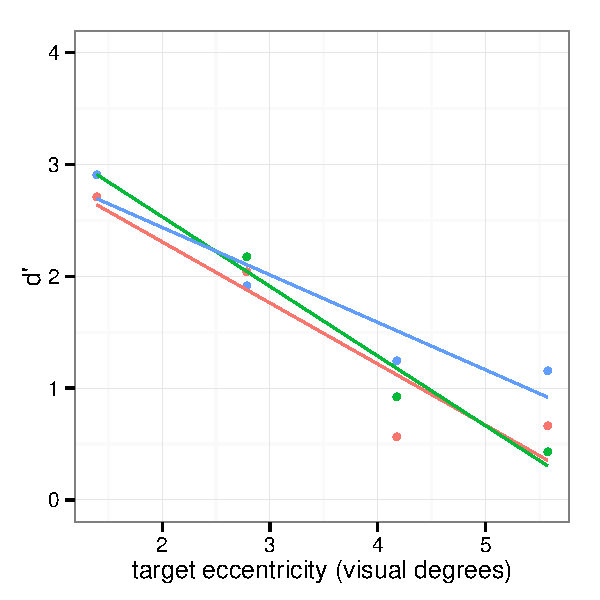
\includegraphics[height=3.6cm]{../dprimeCheck2AFCExp/analysis/dprime.pdf}}
	\subfigure[yes-no]{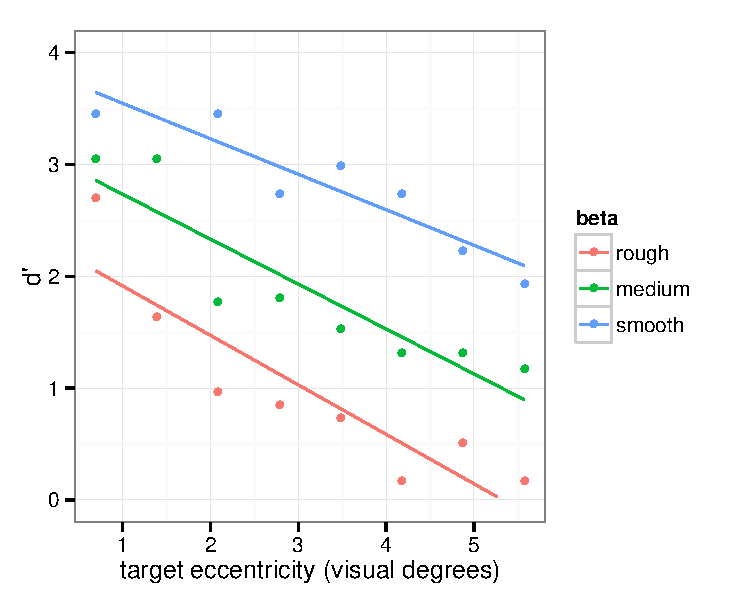
\includegraphics[height=3.6cm]{../dprimeCheck2AFCExp/analysis/YesNo_AllPhi.pdf}}
	\caption{Results from the 2AFC and Yes-No comparison.} 
	\label{fig:2afcResults}	
\end{figure}

We can confirm this difference with a two-way ANOVA. We find that for the 2AFC data, there is statistically significant effect of target eccentricity on $d'$ ($F(1)=67.7$, $p<0.001$) but no significant effect of $\beta$ ($F(2)=0.81$) or interaction ($F(2)=0.80$). However, when looking at the target detection results, we find a statistically significant effect of target eccentricity ($F(1)=70.3$, $p<0.001$) and $\beta$ ($F(2)=54.8$, $p<0.001$). Again, there was no statistically significant interaction ($F(2)=0.09$).

\subsection{Discussion}

We find that the two methods for measuring the target's visibility map give qualitatively different results. The $d'$ scores obtained using two-alternative forced choice appear to be insensitive to changes in surface texture. This is at odds with the results of the visual search data presented in this manuscript (Figure \ref{fig:numFixHumanModel}), and in \textcite{clarke2008, clarke2009} where we can see that surface roughness has a large effect on search difficulty. In particular, we see that the observer had a much higher $d'$ for rough surfaces under the 2afc measurement, which would be expected given the literature on covert attention. For smoother surfaces, the opposite effect is observed. This is potentially due to practise effects. Either way, the implications of under-estimating target visibility for smooth cases is minimal, as observers are already finding the target with only one or two fixations.  


\end{document}